%! TeX program = lualatex
%tags! sr latch toggle flip flop secuencial
\documentclass[letterpaper]{article}
\usepackage[margin=1in]{geometry}
\usepackage{amsmath}
\usepackage{amssymb}
\usepackage{circuitikz}
\usepackage[no-math]{fontspec}
\usepackage[fg,bg]{gruvboxpalette}
\usepackage{hyperref}
\usepackage{newtxsf}
\usepackage[explicit]{titlesec}
\usepackage{tikz}
\usepackage{varwidth}
\usetikzlibrary{calc}
\usetikzlibrary{positioning}
\usetikzlibrary{arrows.meta}
\usepackage[most]{tcolorbox}
\usepackage{tabularray}
\DefTblrTemplate{firsthead, middlehead,lasthead}{default}{}
\DefTblrTemplate{capcont}{default}{}
\DefTblrTemplate{contfoot-text}{normal}{} \SetTblrTemplate{contfoot-text}{normal} \DefTblrTemplate{conthead-text}{normal}{} \SetTblrTemplate{conthead-text}{normal}
\UseTblrLibrary{counter}
\hypersetup{
  colorlinks  = true,
  urlcolor    = Blue,
  linkcolor   = Blue,
  citecolor   = Blue
}
\usepackage[most]{tcolorbox}

\setmainfont{NotoSans-Regular}[
Path           = /home/snouflake/.fonts/ ,
Extension      = .ttf ,
BoldFont       = NotoSans-Bold ,
ItalicFont     = NotoSans-Italic ,
BoldItalicFont = NotoSans-BoldItalic,
] 

\newtcolorbox{defbox}[3][]{%
  colback=blue!30!background,
  coltitle=blue!15!black,
  coltext=font,
  title filled=false,
	enhanced,
  detach title,
  tile,
  before upper={\tcbtitle\medskip\\},
  borderline west={2mm}{0pt}{blue},
  % attach boxed title to top center={yshift=-2mm},
  leftrule=2mm,
  toprule=0mm,
  bottomrule=0mm,
  rightrule=0mm,
  arc=0mm,
	title={Definición:~#2},
	#1
}

\setlength\parindent{0pt}

\usepackage[italic]{mathastext}

\def \T{Sistemas Digitales}
\def \S{Sistemas Secuenciales}

\begin{document}
\begin{tikzpicture}[inner sep=0pt,color=font]
  \node[anchor=west,align=left,line width=0pt] 
    (title) at (0,0) {\huge\bfseries\noindent\T\\\Large\bfseries\S}
    ;
\end{tikzpicture}


\begin{longtblr}{
    colspec={@{}Q[3cm,cmd=\textbf,h] >{\begin{minipage}{\linewidth}}X<{\end{minipage}}@{}},
    rowsep={7pt},
  }
  Flip-Flop SR
  &
  \begin{circuitikz}[thick]
    \draw 
    (1,3) node[nor port, anchor=in 1] (topnor) {}
    (0,3) node[left] {S} to[short] node[midway, above] {0} (topnor.in 1)

    (1,0) node[nor port, anchor=in 2] (botnor) {}
    (0,0) node[left] {R} to[short] node[midway, above] {0} (botnor.in 2)

    (topnor.out) to[short] ++(0,-0.5) to[short] ++(-2,-1) |- (botnor.in 1)

    (botnor.out) to[short] ++(0,0.5) to[short] ++(-2,1) |- (topnor.in 2)

    (topnor.out) node[right] {$\bar{Q}$ ~~ 1}
    (botnor.out) node[right] {$Q$ ~~ 0}
    ;
  \end{circuitikz}
  \bigskip

  \textbf{Tabla de verdad}
  \medskip

  (nunca puede haber $S \& R$, the effects of $S$ or $R$ being true persist when returning to the initial state)
  \medskip

  \begin{tblr}{}
    S & R & Q & $\bar{Q}$ & \\
    \cline[1pt]{1-4}
    0 & 0 &   &   & (initial state) \\
    1 & 0 & 1 & 0 & \\
    0 & 1 & 0 & 1 & \\
    1 & 1 & 0 & 0 & (ungodly, now a race condition)\\
  \end{tblr}

  \bigskip
  \textbf{Versión NAND}{\hspace{10pt}\leavevmode\leaders\hrule height0.42em depth-0.3em\hfill\kern0pt}
  \bigskip

  \begin{circuitikz}[thick]
    \draw 
    (1,3) node[nand port, anchor=in 1] (topnand) {}
    (0,3) node[left] {S} to[short] node[midway, above] {0} (topnand.in 1)

    (1,0) node[nand port, anchor=in 2] (botnand) {}
    (0,0) node[left] {R} to[short] node[midway, above] {0} (botnand.in 2)

    (topnand.out) to[short] ++(0,-0.5) to[short] ++(-2,-1) |- (botnand.in 1)

    (botnand.out) to[short] ++(0,0.5) to[short] ++(-2,1) |- (topnand.in 2)

    (topnand.out) node[right] {$\bar{Q}$ ~~ 1}
    (botnand.out) node[right] {$Q$ ~~ 0}
    ;
  \end{circuitikz}

  \textbf{Tabla de verdad}
  \medskip

  \medskip

  \begin{tblr}{}
    S & R & Q & $\bar{Q}$ & \\
    \cline[1pt]{1-4}
    0 & 0 & 1 & 1 & (now this ones illegal) \\
    1 & 0 & 1 & 0 & \\
    0 & 1 & 0 & 1 & \\
    1 & 1 &   &   & (now this ones then initial state) \\
  \end{tblr}
  \\
  Flip-Flop JK
  &
  \begin{tblr}{}
    $J_t$ & $K_t$ & $Q_{t+1}$ & \\
    \cline[1pt]{1-3}
    0 & 0 & $Q_t$ & (La salida se mantiene igual al siguiente ciclo) \\
    0 & 1 & 0 & \\
    1 & 0 & 1 & \\
    1 & 1 & $\bar{Q_t}$ & (La salida se invierte al siguiente ciclo) \\
  \end{tblr}
  \medskip

  \begin{circuitikz}[thick]
    \draw
      (0,0)
      node[dipchip, hide numbers, num pins=4, draw only pins={1-4}, anchor=north west] (dc) {}

      (dc.bpin 1) node[right] { $J$ }
      (dc.bpin 2) node[right] { $K$ }
      (dc.bpin 3) node[left]  { $\bar{Q}$ }
      (dc.bpin 4) node[left]  { $Q$ }
      ;
  \end{circuitikz}
  \medskip

  \textbf{Diagrama de tiempo}
  \medskip

  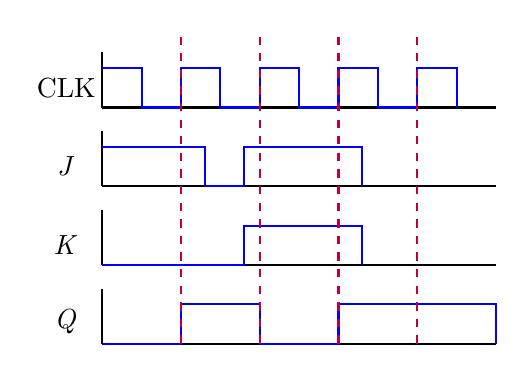
\begin{tikzpicture}[thick]
    \draw[thick]
      (0,4) node[anchor=east,left=13pt,above] {CLK} -- ++(0,0.7)
      (0,3) node[anchor=east,left=13pt,above] {$J$}       -- ++(0,0.7)
      (0,2) node[anchor=east,left=13pt,above] {$K$}       -- ++(0,0.7)
      (0,1) node[anchor=east,left=13pt,above] {$Q$}       -- ++(0,0.7)
      
      (0,1) -- ++(5,0)
      (0,2) -- ++(5,0)
      (0,3) -- ++(5,0)
      (0,4) -- ++(5,0)
      ;
    \draw[thick,blue]
      (0,4.5) -| ++(0.5,-0.5) -| ++(0.5,0.5) -| ++(0.5,-0.5) -| ++(0.5,0.5) -| ++(0.5,-0.5) -| ++(0.5,0.5) -| ++(0.5,-0.5) -| ++(0.5,0.5) -| ++(0.5,-0.5) 

                                   %1.8
      (0,3.5) -| ++(1.3,-0.5) -| ++(0.5,0.5) -| ++(0.2,0) -| ++(1,0) -| ++(0.3,-0.5)

      (0,2) -| ++(1.3,0) -| ++(0.5,0.5) -| ++(0.2,0) -| ++(1,0) -| ++(0.3,-0.5)


      (0,1) -| ++(1,0.5) -| ++(1,-0.5) -| ++(1,0.5) -|  ++(1,0) -| ++(1,-0.5) 
      ;

    \draw[thick,dashed,purple]
      (1,1) -- ++(0,4)
      (2,1) -- ++(0,4)
      (3,1) -- ++(0,4)
      (4,1) -- ++(0,4)
      ;

  \end{tikzpicture}

  \bigskip
  \textbf{Flip-Flop D}{\hspace{10pt}\leavevmode\leaders\hrule height0.42em depth-0.3em\hfill\kern0pt}
  \bigskip

  \begin{tblr}{colspec={
        >{\begin{varwidth}{\linewidth}}c<{\end{varwidth}}
        >{\begin{varwidth}{\linewidth}}c<{\end{varwidth}}
    }}

    \begin{tblr}{}
      $D$ & $Q_{t+1}$ \\
      \cline[1pt]{1-2}
      0 & 0 \\
      1 & 1 \\
    \end{tblr}

    &

    \begin{circuitikz}[thick,american]
      \draw
        (0,0)
        node[dipchip, hide numbers, num pins=4, draw only pins={1-4}, anchor=north west] (dc) {}

        (dc.bpin 1) node[right] { $J$ }
        (dc.bpin 2) node[right] { $K$ }
        (dc.bpin 3) node[left]  { $\bar{Q}$ }
        (dc.bpin 4) node[left]  { $Q$ }

        \pgfextra{\ctikzset{bipoles/not port/width=.4,
            bipoles/not port/height=.15,
        }}
        (dc.pin 1) node[anchor=in, not port, rotate=-90, line width=0.5pt] {} (dc.pin 2)

        (dc.pin 1) to[short] ++(-0.3,0) node[left] {$D$}
        ;
    \end{circuitikz}
  \end{tblr}


  \bigskip
  \textbf{Flip-Flop T}{\hspace{10pt}\leavevmode\leaders\hrule height0.42em depth-0.3em\hfill\kern0pt}
  \bigskip

  \begin{tblr}{colspec={
        >{\begin{varwidth}{\linewidth}}c<{\end{varwidth}}
        >{\begin{varwidth}{\linewidth}}c<{\end{varwidth}}
    }}
    \begin{tblr}{}
      $T$ & $Q_{t+1}$ \\
      \cline[1pt]{1-2}
      0 & $Q$ \\
      1 & $\bar{Q}$ \\
    \end{tblr}

    &

    \begin{circuitikz}[thick,american]
      \draw
        (0,0)
        node[dipchip, hide numbers, num pins=4, draw only pins={1-4}, anchor=north west] (dc) {}

        (dc.bpin 1) node[right] { $J$ }
        (dc.bpin 2) node[right] { $K$ }
        (dc.bpin 3) node[left]  { $\bar{Q}$ }
        (dc.bpin 4) node[left]  { $Q$ }

        (dc.pin 1) to[short] (dc.pin 2)

        (dc.pin 1) to[short] ++(-0.3,0) node[left] {$T$}
        ;
    \end{circuitikz}
  \end{tblr}
  \\


\end{longtblr}
\end{document}
